Dopo aver validato la reattivit\`{a} e la precisione del sensore, in questo capitolo verranno mostrate delle possibili applicazioni 
dei sensori coppia-forza in ambito industriale, con particolare enfasi sulla collaborazione uomo-robot \cite{applications}. 
La prima delle applicazioni che verranno trattate \`{e} un sistema di controllo basato sul feedback di forza che consente ad un 
operatore di muovere il braccio, senza dover utilizzare 
il teach pendant. Nel corso del capitolo verr\`{a} indicata come \textbf{inseguitore di forza}. Tale applicazione \`{e} versatilmente 
adattabile anche per altri scopi, come ad esempio nel task di presa e posizionamento (pick and place), che verr\`{a} trattato come 
secondo esempio di applicazione dei sensori coppia-forza. In tale applicazione, i momenti angolari lungo l'asse z vengono 
utilizzati per indicare al braccio le posizioni da raggiungere per completare con successo il compito assegnato. 
Infine, aggiungendo ulteriori funzionalit\`{a} all'\textit{inseguitore di forza}, verr\`{a} presentato un esempio di trasporto 
collaborativo uomo-robot in cui l'operatore pu\`{o} trasportare in modo sicuro ed efficiente oggetti sottili e leggeri con l'aiuto 
dell'UR5.

\section{Inseguitore di forza} \label{sec:force_follower}
Come accennato, questa applicazione si focalizza sulla necessit\'{a} di poter muovere il robot a piacimento, senza dover 
ricorrere all'utilizzo del teach pendant o RViz\footnotemark{}. 
Diventa di fondamentale importanza se integrata in applicazioni collaborative, per rendere pi\'{u} user friendly l'interfacciamento 
con il robot. 
Quando il sensore rileva delle forze superiori ad una determinata soglia (calcolata sperimentalmente), viene inviato al robot un 
comando \verb|Twist| per farlo muovere con una velocit\'{a} proporzionale alla forza applicata in input. In questo modo, il robot `segue' 
le forze impartite dall'operatore convertendole in termini di velocit\'{a} di movimento. 
Il codice ROS che implementa tale funzionalit\'{a} viene mostrato in \cite{force_follower}. 
Di seguito viene riportato lo pseudocodice. 
\begin{algorithm}[H]
\caption{Inseguitore di forza}\label{algo:force_follower}
\begin{algorithmic}[1]
    \Require $\text{Forze rilevate dal sensore}$
    \Ensure $\text{Comando Twist}$
    \State alpha $\gets$ 200
    \State threshold $\gets$ 5
    \State forces $\gets$ [ ]
    \State twist $\gets$ 0
    %\State valore\_ritornato $\gets$ \textsc{Funzione}\textsc{Prova}(param1, param2)
    
    \While{ros::ok()} 
    \If {$\text{forces.size()} < 20$}
        \State forces.pushback(force) // riempio il vettore con le prime 20 misurazioni
    \Else
        \State forces.erase(forces.begin()) // rimuovo la misurazione meno recente
        \State forces.pushback(force) // per fare spazio all'ultima rilevata
        \State meanVal $\gets$ mean(forces)
        \State moduleVal $\gets$ module(meanVal) 
        \If {$\text{moduleVal} > threshold$}
            \State twist $\gets$ moduleVal / alpha // scalo il valore del modulo
        \Else
            \State twist $\gets$ 0
        \EndIf
        \State publisher.publish(twist)
    \EndIf
    \State ros::speedOnce()
    \EndWhile
\end{algorithmic}
\end{algorithm}
\footnotetext{\url{https://github.com/andreastocco01/ur5_ft_tasks/blob/main/src/velocity_force_follower.cpp}}
Dopo aver portato il robot in posizione di partenza con MoveIt, viene attivato \verb|twist_controller| con la stessa funzione 
utilizzata nell'esperimento del burro d'arachidi (presente in \verb|utils.cpp|).  
All'interno del vettore \verb|forces| vengono salvate le ultime 20 misurazioni del sensore. Di queste ne viene calcolata la media 
e, se il modulo \'{e} superiore alla soglia specificata, viene inviato al robot un comando \verb|Twist| contenente uno scalamento delle 
forze rilevate nelle tre componenti. Il calcolo della velocit\'{a} di movimento viene fatto sulla media degli ultimi campioni 
per una questione di utilizzabilit\'{a}. Servirsi delle misurazioni singole per il calcolo del vettore velocit\'{a} da inviare al robot 
porta ad un movimento poco fluido e impulsivo che peggiora l'esperienza utente. 
Utilizzando la media, invece, le piccole variazioni 
di forza generate dall'operatore vengono ammortizzate portando ad una risposta da parte del braccio pi\'{u} naturale.
La conversione tra forza e velocit\'{a} avviene mediante un'attenuazione delle componenti del vettore media per un coefficiente 
costante. In questo modo si riduce l'influenza delle forze `piccole' nel vettore velocit\'{a} risultante, valorizzando maggiormente le 
componenti pi\'{u} ampie. 

\section{Pick and place} \label{sec:pick_place}
Il pick and place \'{e} un'applicazione largamente utilizzata in ambito industriale e consiste nello spostamento di un oggetto 
da un punto di partenza ad uno di destinazione. Tale compito pu\'{o} essere portato a termine senza l'ausilio di un sensore 
coppia-forza. L'alternativa proposta in questa tesi si concentra su uno scenario di collaborazione uomo-robot, in cui l'operatore 
insegna al robot dove si trova il pezzo da raccogliere e dove dovr\'{a} essere posizionato. 
Per fare ci\'{o} si \'{e} reso necessario installare un gripper come end effector 
dell'UR5 \cite{gripper_repo}. In \cite{environment_setup} con MoveIt Setup Assistant \'{e} stata generata la cartella contenente 
tutti i file di configurazione per questo specifico setup. 
% mettere immagine di RViz
In Figura \ref{fig:pick_place} viene mostrato l'ambiente di lavoro comprensivo del gripper per la presa degli oggetti. 
\begin{figure}[H]
    \centering
    \includegraphics*[width=0.65\textwidth]{images/pick_place_setup.jpg}
    \caption{Setup applicazione pick and place}
    \label{fig:pick_place}
\end{figure}
Inizialmente il robot apprende il punto di partenza e di destinazione dall'operatore, poi, una volta preso l'oggetto, 
proceder\'{a} con la sua collocazione nella posizione finale.
Di seguito verranno descritte le parti in cui \'{e} stata suddivisa l'applicazione.
\subsection{Salvataggio delle posizioni} \label{sub:positions}
Inizialmente, viene utilizzato l'\textit{inseguitore di forza} per il salvataggio delle posizioni di partenza e di destinazione 
su cui il robot dovr\'{a} spostarsi per portare a termine il proprio compito. 
L'operatore potr\'{a}, quindi, muovere il braccio liberamente fino a quando non si trova al di sopra dell'oggetto da spostare. 
\'{E} stata implementata una gesture che consiste nell'applicazione di una piccola torsione al sensore, 
per salvare la posizione attuale in cui si trova il robot, corrispondente al punto in cui si trova l'oggetto. Il gripper 
si aprir\'{a} e si chiuder\'{a} velocemente per indicare che la posizione \'{e} stata salvata correttamente nel vettore 
\verb|positions|. Di seguito viene riportato lo pseudocodice per questa funzionalit\'{a}.
\begin{algorithm}[H]
    \caption{Salvataggio posizioni}\label{algo:positions}
    \begin{algorithmic}[1]
        \Require $\text{Forze e momenti rilevati dal sensore}$
        \Ensure $\text{Vettore di posizioni}$
        \State torqueThreshold $\gets$ 1
        \State forces $\gets$ [ ]
        \State positions $\gets$ [ ]
        
        \While{ros::ok() \textbf{and} $\text{positions.size()} < 3$} 
            \If {$\text{forces.size()} < 20$}
                \State forces.pushback(force) // riempio il vettore con le prime 20 misurazioni
            \Else

                // codice inseguitore di forza
                \If{$\text{abs(torque).z} > \text{torqueThreshold}$}
                    \State positions.pushback(currentPosition)
                    \State feedback()
                \EndIf
                \State twistPublisher.publish(twist)
            \EndIf
            \State ros::speedOnce()
        \EndWhile
        \State posPublisher.publish(positions[0])
        \State posPublisher.publish(positions[1])
    \end{algorithmic}
    \end{algorithm}
Lo stesso dovr\'{a} essere fatto anche per la posizione di destinazione e per una posizione fittizia in una zona libera 
del piano di lavoro (vedi \ref{sub:placement}). Una volta terminata la fase di acquisizione delle posizioni, 
le prime due verranno pubblicate sul topic \verb|task_positions|.
\subsection{Posizionamento} \label{sub:placement}
In questa fase, il nodo \textbf{placement}\footnotemark{} potr\'{a} iscriversi al topic e leggere le posizioni precedentemente 
acquisiste. Inizialmente, dalla posizione fittizia, il robot scender\'{a} verso il basso fino a quando non verr\'{a} rilevata 
una forza lungo l'asse z, corrispondente al contatto con il piano di lavoro. Tale posizione verr\'{a} salvata e utilizzata in seguito. 
Con MoveIt il braccio viene spostato alla prima posizione del topic, ossia il punto in cui \'{e} presente l'oggetto da prendere.
Da qui, si muover\'{a} verso il basso alla ricerca di un contatto con esso e una nuova posizione verr\'{a} salvata. 
Le differenza delle due posizioni corrisponde all'altezza dell'oggetto. Sar\'{a}, dunque, sufficiente chiudere il gripper 
nel suo punto medio per favorirne una presa pi\'{u} solida. Ad esempio, se l'oggetto \'{e} alto 10 cm, il gripper verr\'{a} chiuso 
ad altezza 5 cm. 
L'UR5, poi, si muover\'{a} nell'altra posizione pubblicata sul topic in attesa di cominciare l'ultima fase dell'applicazione.
\footnotetext{\url{https://github.com/andreastocco01/ur5_ft_tasks/blob/main/src/placement.cpp}}
\subsection{Inserimento} \label{sub:insertion}
Supponendo di voler inserire l'oggetto in un contenitore avente, al centro, una cavit\'{a} di uguale forma e di dimensioni simili, 
non sar\'{a} sufficiente utilizzare la posizione acquisita grossolanamente in \ref{sub:positions}, in quanto troppo poco precisa. 
A tal proposito viene mostrato il codice per calcolare il centro del contenitore (corrispondente al 
centro della cavit\'{a}) in cui inserire l'oggetto\footnotemark{}. Utilizzando il controllore di velocit\'{a} il braccio viene fatto muovere 
finch\'{e} non viene rilevato un contatto con tutti i bordi. Vengono salvate le posizioni di ogni estremit\'{a} e vengono, poi, 
utilizzate per calcolare il punto esatto in cui inserire l'oggetto. Il robot potr\'{a}, quindi, posizionarsi al di sopra di 
tali coordinate e cominciare un processo di discesa che lo porter\'{a} ad inserire l'oggetto precisamente nell'alloggiamento finale, 
come mostrato in Figura \ref{fig:insertion}. 
\footnotetext{\url{https://github.com/andreastocco01/ur5_ft_tasks/blob/main/scripts/place_ontop.py}}
\newpage
\begin{figure}[H]
    \centering
    \includegraphics*[width=0.65\textwidth]{images/insertion.jpg}
    \caption{Fase di inserimento}
    \label{fig:insertion}
\end{figure}


\subsection{Movimento a spirale}
Una possibile variazione del pick and place consiste nel far si che il braccio \textbf{trovi} la cavit\`{a} in cui inserire l'oggetto. 
In \ref{sub:insertion} si presupponeva che la cavit\`{a} si trovasse al centro del contenitore, in questo modo era possibile, 
determinandone il centro, inserire precisamente l'oggetto nella posizione corretta. Ovviamente se il foro non si trova al centro, 
l'inserimento non andr\`{a} a buon fine. Per risolvere questo problema si \`{e} pensato di sostituire la parte di inserimento 
precedentemente descritta con un nuovo nodo in grado di trovare la posizione del foro\footnotemark{}. 
In Figura \ref{fig:spiral_pick_place} viene mostrato come, in questo caso, il foro in cui inserire l'oggetto non sia pi\`{u} al centro 
del contenitore, bens\`{i} in basso a destra. 
\footnotetext{\url{https://github.com/andreastocco01/ur5_ft_tasks/blob/main/src/spiral_movement.cpp}}
\newpage
\begin{figure}[H]
    \centering
    \includegraphics*[width=0.35\textwidth]{images/spiral_pick_place.jpg}
    \caption{Setup pick and place con movimento a spirale}
    \label{fig:spiral_pick_place}
\end{figure}
Per la ricerca dell'esatta posizione del foro, si assume nota una posizione grossolana da cui partire. 
Il braccio è quindi portato in tale posizione e fatto scendere fino al contatto con il contenitore.
Da qui il robot, comincia ad effettuare un movimento a \textbf{spirale}. 
Mentre effettua tale movimento, mantiene l'oggetto in contatto con la superficie del contenitore. Se il sensore 
non rileva pi\`{u} alcuna forza lungo l'asse z, significa che ci si trova in uno dei seguenti casi:
\begin{itemize}
    \item il contenitore non ha una superficie piana. Il foro non \`{e} ancora stato trovato e quindi \`{e} necessario far scendere 
    il braccio per ristabilire il contatto e continuare a cercare.
    \item il braccio si trova al di sopra del foro. Si pu\`{o} procedere con l'inserimento dell'oggetto.
\end{itemize} 
Per implementare questa funzionalit\`{a} si \`{e} pensato di far scendere il braccio ogni qual volta il sensore non rileva pi\`{u}
una forza lungo l'asse z, come mostrato in Algorithm \ref{algo:spiral}. 
\newpage
\begin{algorithm}[H]
    \caption{Movimento a spirale}\label{algo:spiral}
    \begin{algorithmic}[1]
        \Require $\text{Forze rilevate dal sensore}$
        \Ensure $\text{Inserimento dell'oggetto}$
        \State threshold $\gets$ -8
        \State lim $\gets$ 0.02
        \State twist $\gets$ 0
        \State firstTime $\gets$ true
        \State height
        
        \Repeat 
            \While{$\text{force.z} > \text{threshold}$}
                \State twist $\gets$ (0, 0, -0.015) // vado gi\`{u} finch\`{e} non c'\`{e} un contatto
                \State publish(twist)
            \EndWhile
            \State twist $\gets$ 0
            \State publish(twist) // mi fermo
            \If{firstTime}
                \State heigth $\gets$ currentPosition // salvo l'altezza del contenitore
                \State firstTime $\gets$ false
            \EndIf
            \State currentHeight $\gets$ currentPosition
            \While{$\text{force.z} \leq \text{threshold}$ \textbf{and} $\text{height} - \text{currentHeight} < \text{lim}$}

                // movimento a spirale
            \EndWhile
        \Until{$\text{force.z} > \text{threshold}$ \textbf{and} $\text{height} - \text{currentHeight} < \text{lim}$}
    \end{algorithmic}
    \end{algorithm}
Se la differenza di altezza \`{e} superiore ad una determinata soglia, significa che probabilmente si \`{e} 
trovato il foro e quindi il gripper si aprir\`{a} per favorire l'inserimento dell'oggetto. 
A differenza della versione mostrata in \ref{sec:pick_place}, questa non raggiunge sempre l'obiettivo. 
Pu\`{o} capitare, infatti, che il braccio non trovi mai la cavit\`{a} per via dell'incremento del raggio della spirale e che finisca 
al di l\`{a} dei bordi della scatola. Inoltre, se non si trova perfettamente al di sopra del foro, potrebbe non cominciare la 
fase di discesa non portando cos\`{i} a termine il compito. 
In Figura \ref{fig:spiral_insertion}, il quadrato centrale indica il foro in cui inserire l'oggetto, mentre le croci individuano i 
punti da cui \`{e} stato fatto partire il movimento a spirale nei vari test effettuati. 
\begin{figure}[H]
    \centering
    \includegraphics*[width=0.65\textwidth]{images/spiral.png}
    \caption{Test effettuati}
    \label{fig:spiral_insertion}
\end{figure}
Nella tabella vengono mostrati i risultati nei vari casi
\begin{center}
    \begin{tabular}{ ||c|c|| } 
     \hline
     Test & Esito\\
     \hline\hline 
     (1) & \ding{51} \\ 
     (2) & \ding{51} \\ 
     (3) & \ding{55} \\ 
     (4) & \ding{51} \\ 
     (5) & \ding{55} \\ 
     \hline
    \end{tabular}
\end{center}
Come gi\`{a} anticipato, con questa applicazione non si ottengono sempre i risultati sperati. In (3) il robot ha cominciato il 
movimento troppo vicino al bordo del contenitore ed \`{e} andato oltre ad esso. In (5), invece, l'interferenza degli altri fori 
ha fatto s\`{i} che si incastrasse senza raggiungere l'obiettivo.


\section{Trasporto collaborativo}
Modificando ulteriormente l'\textit{inseguitore di forza} si pu\'{o} implementare un'applicazione 
per il trasposto collaborativo uomo-robot\footnotemark{}. 
In tale applicazione uomo e robot collaborano per muovere una lamina in fibra di carbonio da una posizione iniziale fino ad uno stampo 
di lavorazione: l'operatore tiene un lembo del materiale mentre il robot tiene l'altra estremit\'{a} attraverso una ventosa. 
L'operatore, tirando a s\'{e} la lamina, fa s\'{i} che il robot segua le sue intenzioni di movimento agevolando lo spostamento del materiale.
Rispetto alla versione utilizzata nella Sezione \ref{sec:force_follower} \'{e} stata aggiunta 
la lettura delle torsioni misurate dal sensore. 
Ad esempio, nel pick and place, le torsioni lungo l'asse z venivano interpretate come l'input da parte dell'operatore per il salvataggio 
delle posizioni. In questo caso, invece, quando il sensore misura una torsione, essa viene interpretata come la volont\'{a} 
dell'operatore di ruotare il pezzo che viene trasportato.
Allo stesso modo delle forze, viene calcolata la \textbf{velocit\'{a} angolare} 
con cui far ruotare l'end effector dell'UR5, in modo tale da riuscire a seguire tutte le intenzioni dell'utente. 
La possibilit\'{a} di rotazione dell'end effector porta, per\'{o}, ad un problema con i sistemi di riferimento. 
Infatti, \verb|twist_controller|, effettua i movimenti rispetto al sistema di riferimento dell'end effector, ma se esso viene ruotato 
sar\'{a} necessario cambiare il verso di movimento per seguire correttamente le forze in input. Per ovviare a questo 
problema, sono state utilizzate le \textbf{trasformazioni geometriche} da un sistema di riferimento ad un altro \cite{foote2013tf}. 
Utilizzando la libreria \verb|tf| di ROS, \'{e} possibile convertire le coordinate di un punto in un sistema di riferimento, nelle 
coordinate di un altro sistema di riferimento connesso ad esso. In questo modo \'{e} stato possibile inviare i comandi 
\verb|Twist| al robot, rispetto ad un sistema di riferimento fisso (quale la base del robot), in modo tale che il vettore velocit\'{a} 
calcolato non fosse dipendente dall'orientazione dell'end effector. 
In questa applicazione si \'{e} sostituito il gripper con delle ventose collegate ad un compressore che, attraverso la creazione di 
una forza di aspirazione, permette al robot di sollevare oggetti sottili e fragili come una lamina di carbonio (vedi Figura \ref{fig:co-op}).
\begin{figure}[H]
    \centering
    \begin{subfigure}[b]{0.45\textwidth}
        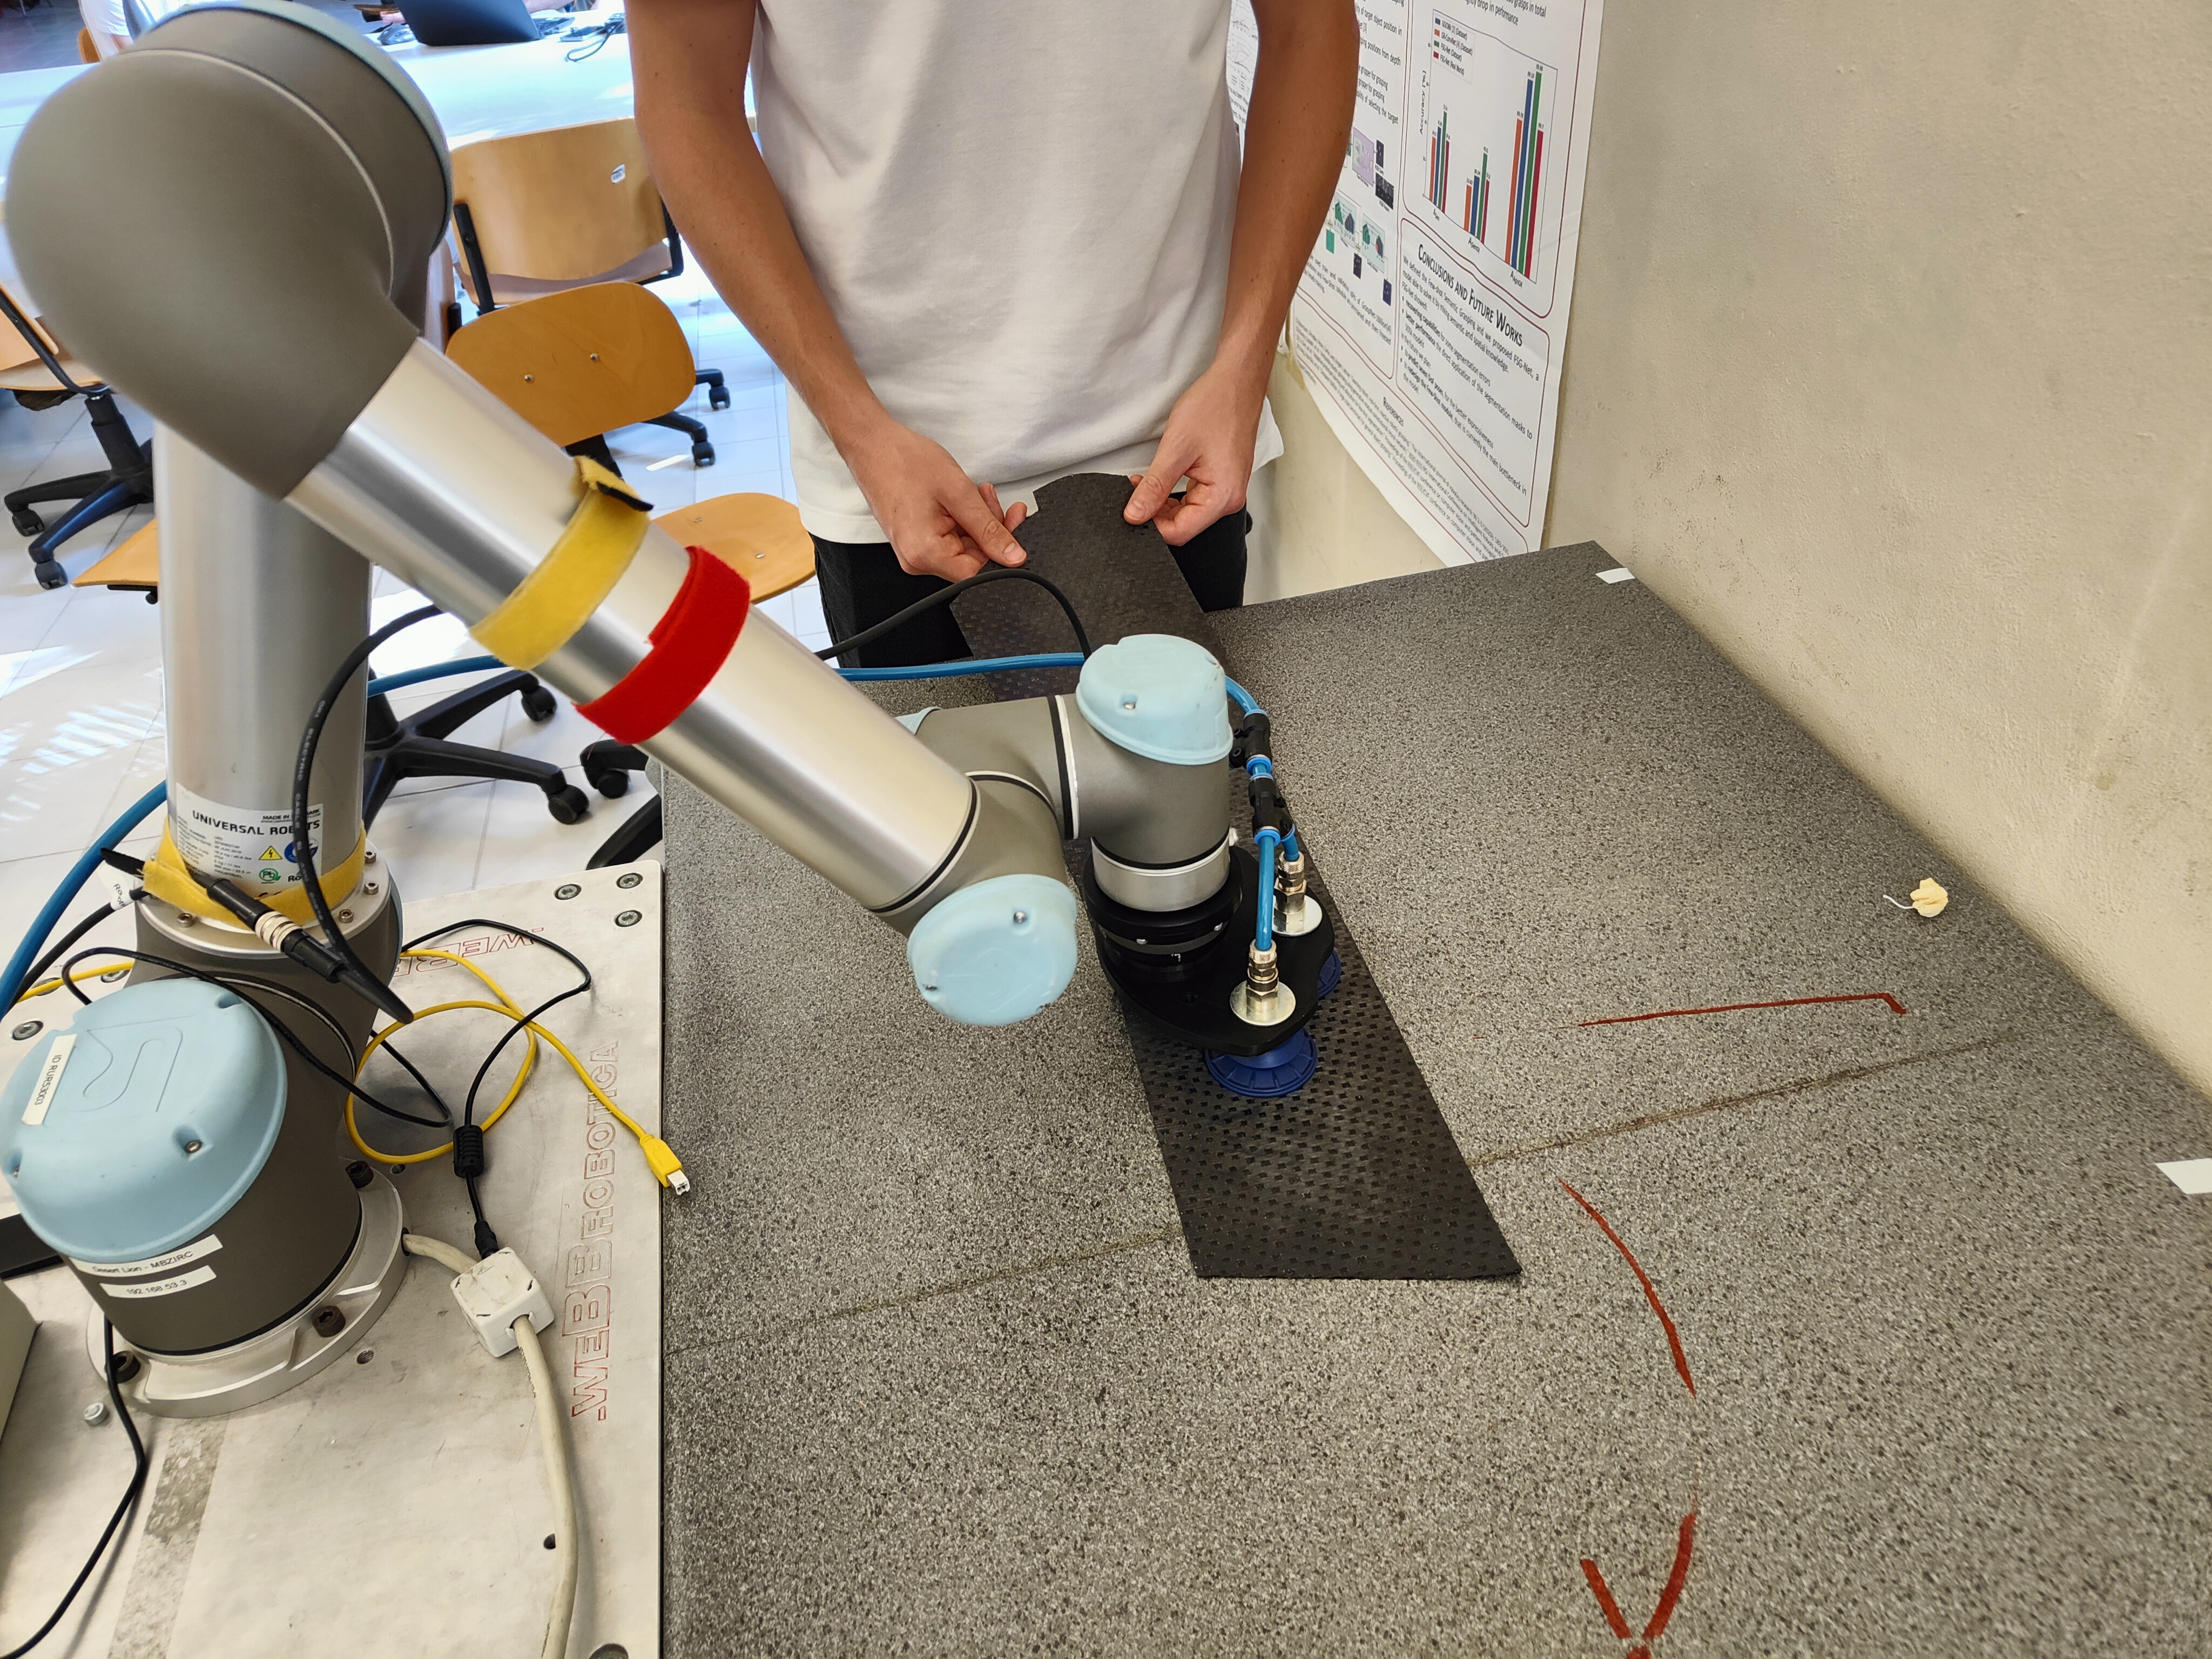
\includegraphics[width=\textwidth]{images/co-op1.jpg}
        \label{fig:co-op1}
    \end{subfigure}
    \qquad
    \begin{subfigure}[b]{0.45\textwidth}
        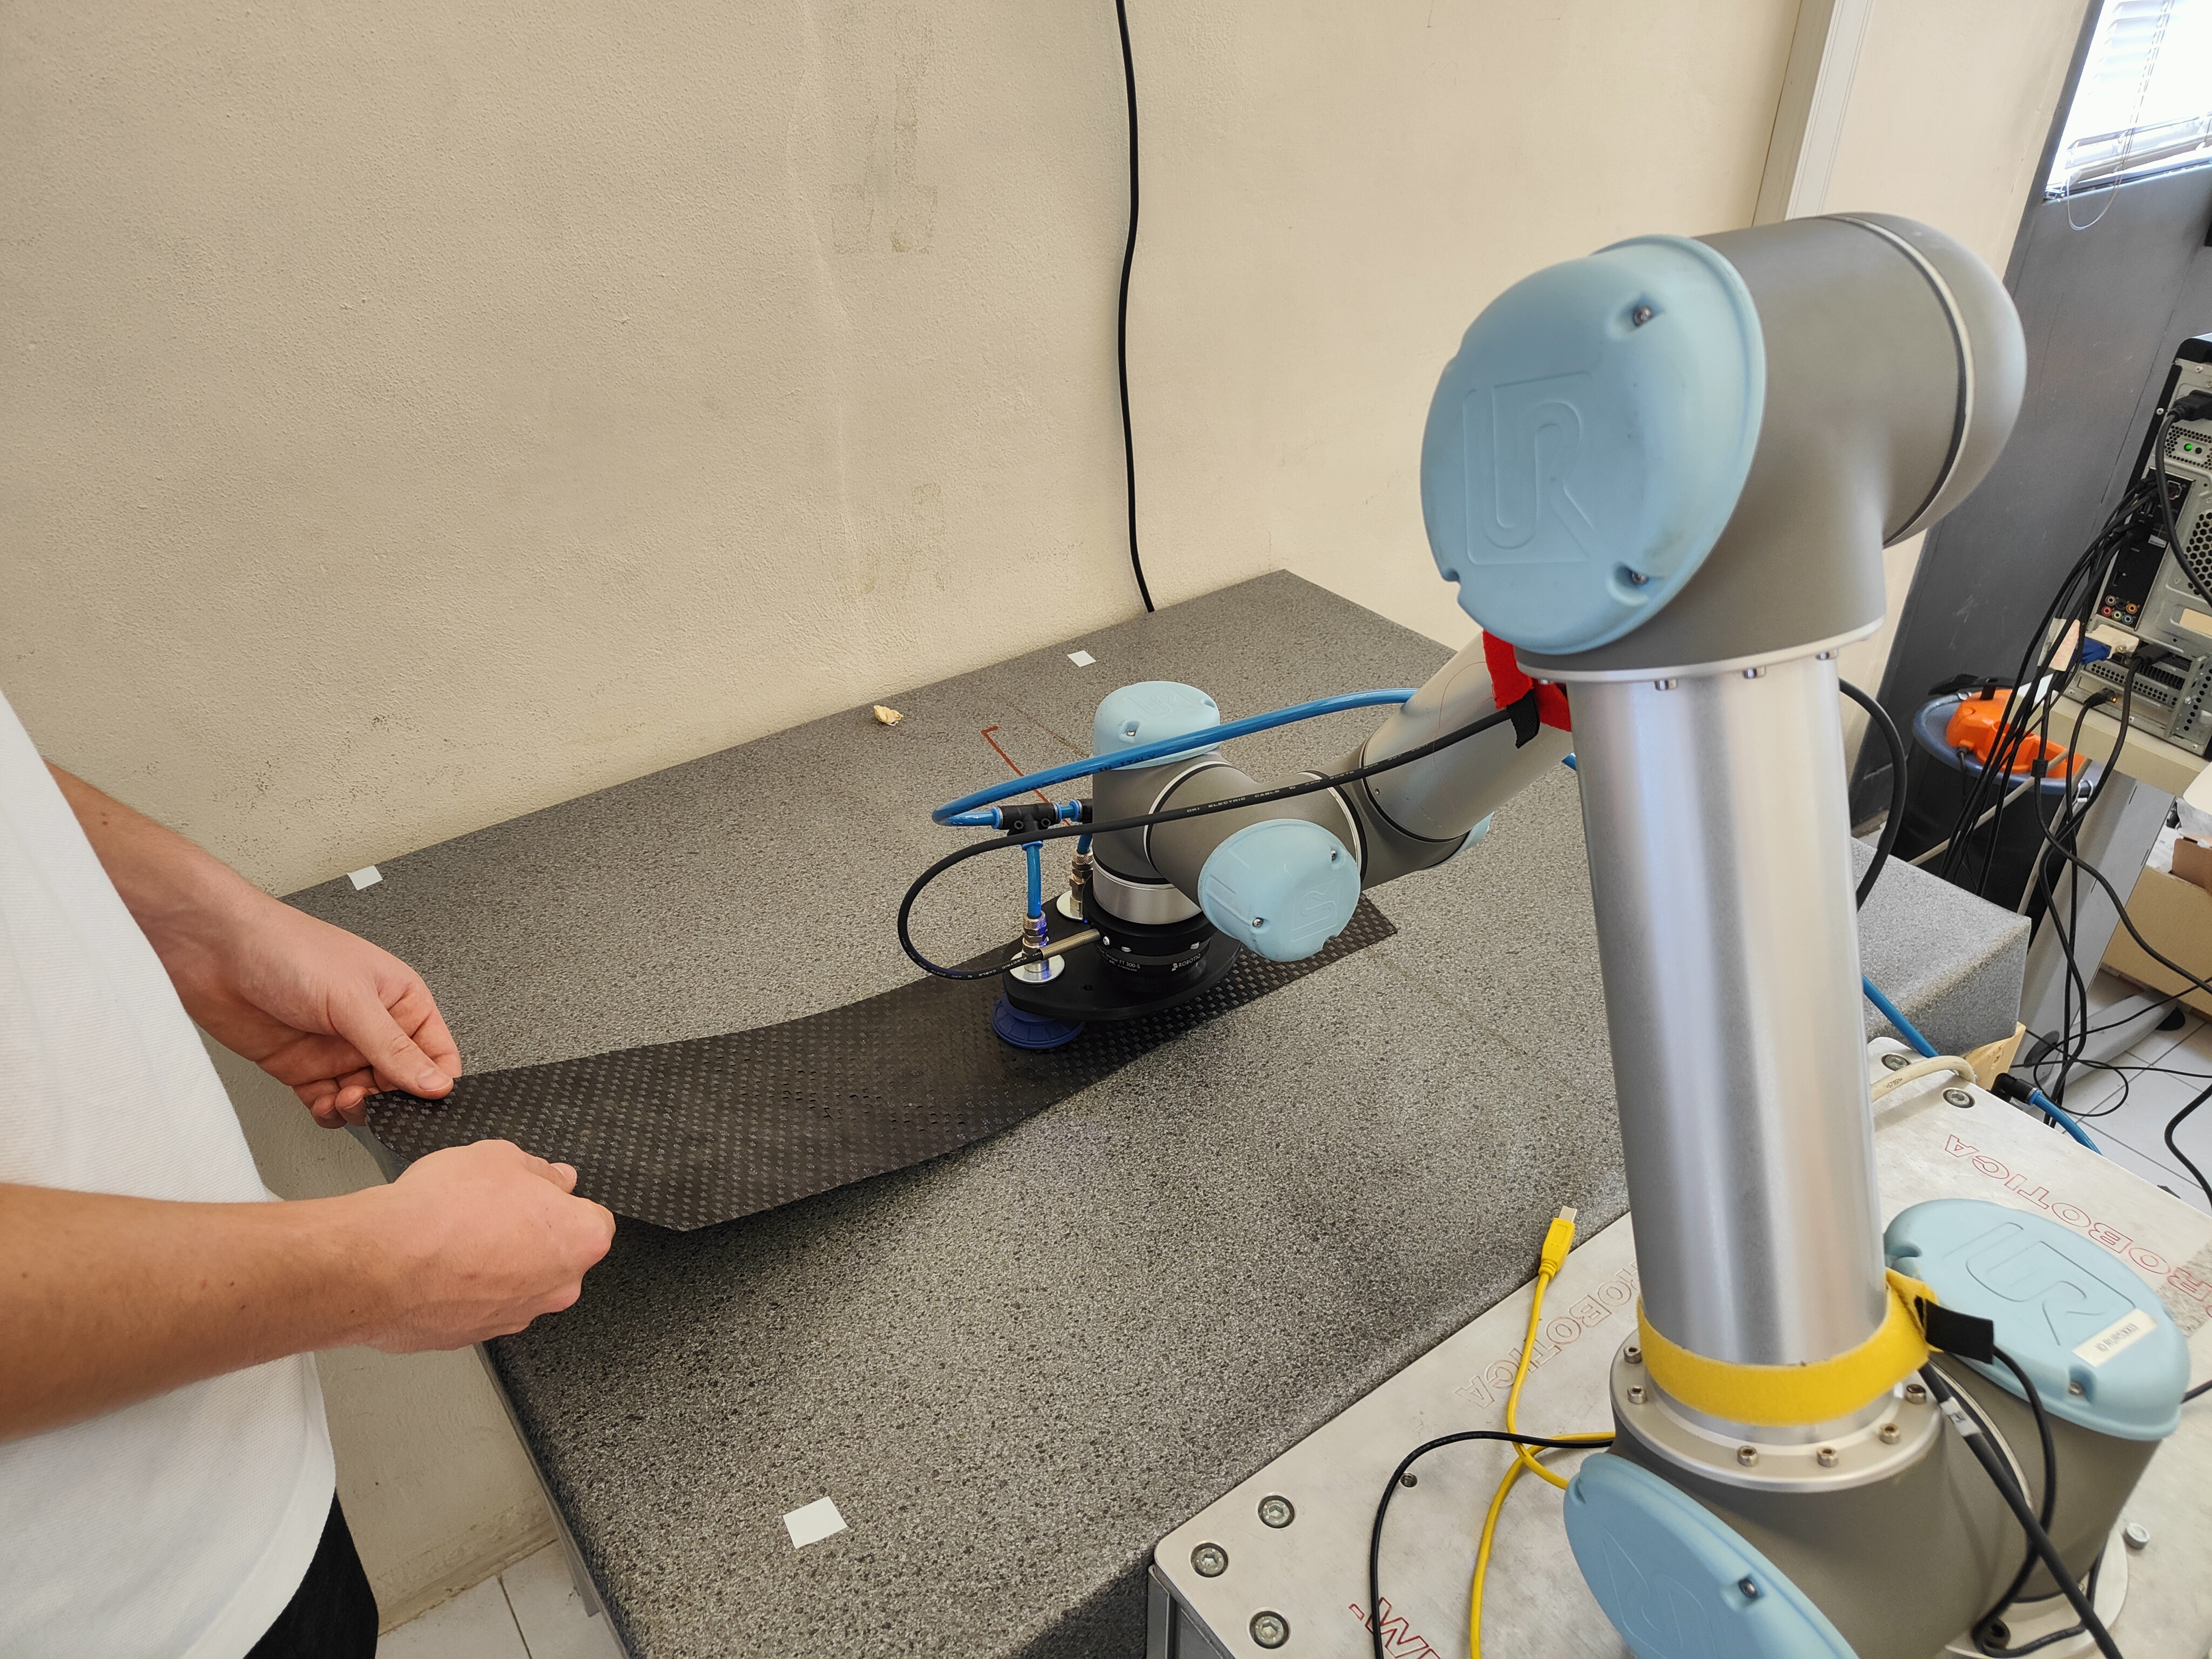
\includegraphics[width=\textwidth]{images/co-op2.jpg}
        \label{fig:co-op2}
    \end{subfigure}
    \caption{Applicazione di trasporto collaborativo, dove il robot segue i movimenti della persona in base alla lettura del sensore di forza}\label{fig:co-op}
\end{figure}
Con l'ausilio dell'\textit{inseguitore di forza}, si potr\'{a} poi trasportare e ruotare la lamina in collaborazione con il robot. 
\footnotetext{\url{https://github.com/andreastocco01/ur5_ft_tasks/blob/main/src/full_velocity_force_follower.cpp}}
